\documentclass[12pt]{report}
\usepackage[spanish]{babel}
\usepackage[utf8]{inputenc}
\usepackage{graphicx}
\usepackage{verbatim}
\usepackage{listings}
\usepackage{float}
\renewcommand*\thesection{\arabic{section}}

\begin{document}
	
	\begin{center}
		\textbf{Análisis de Algoritmos, Sem: 2018-1, 3CV1, Práctica 9, 11-2017}
		\newline
	\end{center}
	
	\begin{center}
		\begin{picture}(0,0) \put(-125,-55){
			\includegraphics[width=2.7cm]{../../IPNlogo.jpg}} 
		\end{picture}
		\LARGE Escuela Superior de Cómputo.\\
		Instituto Politécnico Nacional, México.\\
		\begin{picture}(0,0) \put(160,10){
			\includegraphics[width=2.7cm]{../../logoescom.png}} 
		\end{picture}
	\end{center}
	
	\begin{center}
		\Large Práctica 9: Estrategia Greedy.\\
	\end{center}
	
	\begin{center}
		\textbf{Blancas Pérez Bryan Israel}\\
		orionmunecaycanica@gmail.com\\
	\end{center}
	
	
	\textbf{\large Resumen: }Implementar un algoritmo basado en la estrategia Greedy. El algoritmo a implementar, será el "algoritmo de Huffman" para la contrucción de "códigos de Huffman", utilizado para la compresión de archivos. \newline\\
	\textbf{\large Palabras Clave: } Huffman, Código Huffman, Algoritmos Greedy, Complejidad Computacional.\\
	

	\section{Introducción}
	\textbf{Algoritmos Greedy.}\\
	También conocidos como Algoritmos Voraces, los algoritmo Greedy, son aquellos que, para resolver un problema determinado, sigue un esquema de resolución consistentes en elegir la solución óptima en cada paso local, con la esperanza de llegar a la solución general óptima. Gracias a esta forma de resolución del problema, los algoritmos greedy son algoritmos muy fáciles de diseñar. [1] \\ 
	Es decir, contrario a la programación dinámica, un algoritmo voraz, nunca tomará en cuenta la decisión que se tomó previamente, a este tipo de algoritmos sólo les interesa elegir la mejor solución en el momento actual, o dicho de otra forma, sólo les interesa elegir la mejor opción en esa etapa de la resolución del problema.
	
	\newpage
	
	\section{Conceptos Básicos}
	\textbf{Codificación Huffman}\\
		
	La codificación Huffman es un algoritmo utilizado para la compresión de datos. Fue desarrollado por David A. Huffman mientras estudiaba su doctorado en la MIT, en 1952. Esta codificación hace uso del algoritmo Huffman, el cual es un algoritmo voraz.[2]\\ 
	
	\textbf{Vista general del funcionamiento del algoritmo Huffman.}\\
	
	El algoritmo trabaja a partir de un conjunto de símbolos con sus respectivos pesos (repeticiones) dado. El algoritmo consiste en la creación de un árbol binario que tiene cada uno de los símbolos del alfabeto de entrada como hoja, y construido de manera que no sea ambiguo, para después asignar códigos de distinta longitud de bits a cada uno de los simbolos. Una cosa que vale la pena resaltar, es que mientras mas común (aparece con más frecuencia) sea el símbolo, menor es la cantidad de bits que se le asigna, de tal forma que el símbolo con más repeticiones, es también, el que menor cantidad de bits tiene asignado en la codificación.\\
	
	\textbf{Pasos del algoritmo:}\\
	\textbf{1.} A partir de la tabla de frecuencias de los símbolos, crear una lista con cada tupla de la tabla, y ordenar la lista crecientemente considerando la frecuencia del símbolo.\\
	\textbf{2.} Convertir cada elemento de la lista en un árbol.\\
	\textbf{3.} Fusionar todos los árboles en uno solo:\\
	\textbf{3.1.} Con los dos primeros árboles formar un nuevo árbol, cada uno de los árboles originales en una rama.\\
	\textbf{3.2.} Sumar las frecuencias de cada rama en el nuevo elemento árbol.\\
	\textbf{3.3.} Insertar el nuevo árbol en el lugar adecuado de la lista según la suma de frecuencias obtenida.\\
	\textbf{4.} Para asignar el nuevo código binario de cada carácter sólo hay que seguir el camino adecuado a través del árbol. Si se toma una rama cero, se añade un cero al código, si se toma una rama uno, se añade un uno.\\
	\textbf{5.} Se recodifica el fichero según los nuevos códigos.\\
	
	\newpage
	
	\textbf{Pasos para la decodificación del archivo:}\\
	\textbf{1. }Cargar la codificación a la memoria.\\
	\textbf{2. }Empezar a leer bits del archivo binario.\\
	\textbf{3. }Leer bits de uno en uno, y checar si la cadena de bits está en la codificación.\\
	\textbf{4. }Si se encuentra la cadena de bits en la codificación, escribir el símbolo correspondiente en el archivo de salida.\\
	
	
	

	\section{Experimentación y Resultados}	
	\textbf{Ejercicio 1.}\\
Implementar el algoritmo de la codificación de Huffman con las siguientes condiciones:\\

\textbf{Para la codificación:}\\

\textbf{Entrada}: Un archivo de texto con extensión .txt (original.txt) a codificar.\\

\textbf{Salida}: se generaran tres archivos .txt.\\
\textbf{Frecuencias.txt}: Mostrará la tabla de frecuencias de los caracteres que
aparecen en el archivo original.txt.\\
\textbf{Codificacion.txt}: Mostrará los caracteres que aparecen en el archivo
original.txt y la codificación que le corresponde.\\
\textbf{Archivo\_codificado.txt}: Mostrará el archivo codificado.\\

\textbf{Para la decodificación:}\\

\textbf{Entrada}: \textbf{Archivo\_codificado.txt} generado en la codificación y los archivos necesarios para su decodificación.\\

\textbf{Salida}: Mostrar la información decodificada (\textbf{archivo\_decodificado.txt}).\\

 \newpage
	
	Pseudocódigo del algoritmo:
	\lstset{language=python, breaklines=true, basicstyle=\footnotesize}
	\lstset{numbers=left, numberstyle=\tiny, stepnumber=1, numbersep=10pt}
	\begin{lstlisting}
#Funciones Auxiliares

def existLetter(letters, char):
  k=0
  for node in letters:
    if (node[1]==char):
      return k 
    k+=1
  return -1

def getFrecuency(i):
  letters=[]
  k=0
  for line in i:
    for char in line:
      k=existLetter(letters,char)
      if (k==-1):
        letters.append([1,char])
      else:
        aux=letters[k]
        aux[0]+=1
        letters[k]=aux
  return letters

#Algoritmo de Huffman

def encode(letters):
  heap=[[frecuence,[char, '']] for frecuence, char in letters]
  heapify(heap)

  while (len(heap)>1):
    x=heappop(heap)
    y=heappop(heap)

    for i in x[1:]:
      i[1]='0'+i[1]
    for i in y[1:]:
      i[1]='1'+i[1]

    heappush(heap,[x[0]+y[0]]+x[1:]+y[1:])

  return heappop(heap)

	\end{lstlisting}
	
	\newpage

Función \textbf{getFrecuency} retorna, en forma de lista, la frecuencia de los símbolos del archivo introducido; hace uso de la función \textbf{existLetter} para saber si un símbolo ya había sido tomado en cuenta, para así aumentarle el contador de la frecuencia, o por el contrario, agregar un nuevo elemento a la lista.\\
La función \textbf{encode}, es la implementación del algoritmo de Huffman, descrito en la sección anterior. Esta función realiza exactamente los mismos pasos que el algoritmo descrito con anterioridad. Los métodos utilizados, pertenecen a una librería llamada \textbf{heapq}, disponible en lenguaje python, la cual nos brinda una forma alternativa de implementar las estructuras de datos necesarias para el algoritmo (árbol binario), mediante una cola de prioridades.\\

\textbf{Ejecución del Algoritmo.}\\
	
	\textbf{Input}.\\
	La figura 1, muestra el contenido del archivo \textbf{original.txt}: 
		\begin{figure}[H]
			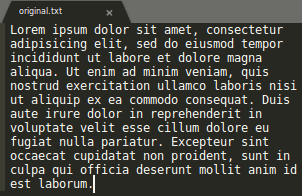
\includegraphics[width=10cm]{imagenes/1.png}
			\centering
			\caption{Original.txt.}
			\centering
		\end{figure}	
		
		\newpage 
		
	\textbf{Output}.\\	
La figura 2, muestra la tabla de frecuencias generada por el algoritmo en el archivo \textbf{frecuencias.txt}:
	\begin{figure}[H]
		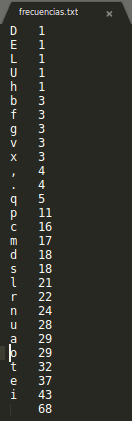
\includegraphics[height=6cm]{imagenes/2.png}
		\centering
		\caption{frecuencias.txt.}
		\centering
	\end{figure}
	
La figura 3, muestra la tabla de codificación generada por el algoritmo en el archivo \textbf{codificacion.txt}, cabe resaltar que como se muestra en la figura 2, los símbolos con más repeticiones (i, \textit{espacio}), son los que tiene menor número de bits en su correspondiente código:
\begin{figure}[H]
	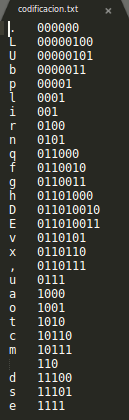
\includegraphics[height=6cm]{imagenes/3.png}
	\centering
	\caption{codificacion.txt.}
	\centering
\end{figure}
	  \newpage
	  
La figura 4, muestra la codificación generada por el algoritmo en el archivo \textbf{archivo\_codificado.txt}:
\begin{figure}[H]
	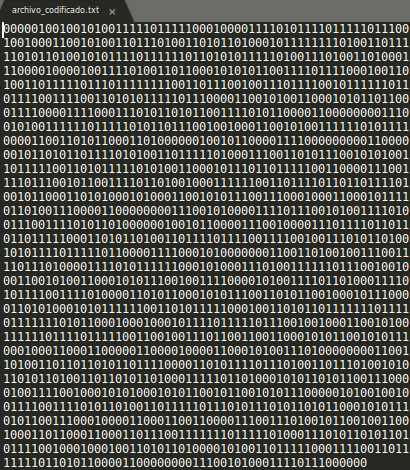
\includegraphics[height=6cm,width=8cm]{imagenes/4.png}
	\centering
	\caption{archivo\_codificado.txt.}
	\centering
\end{figure}

Cabe aclarar que, con motivos de visibilidad para el humano, el archivo resultante imprime ya sea '0' o '1', pero en formato ASCII, por lo que el archivo resultante es más \textit{pesado} que el original. Ejemplo: en la tabla de codificación se muestra que el símbolo \textit{i}, tiene un código asignado igual a '001', el cual representa unicamente 3 bits, menor a el byte necesario para expresar \textit{i} en código ASCII, sin embargo, al momento de imprimir en el archivo \textbf{archivo\_codificado.txt}, es necesario imprimir un bit en formato ASCII, para que sea legible al humano, lo que representa que cada bit terminará \textit{pesando} un byte. Para arreglar eso, mediante programación he obtenido el peso de la compresión, contando el número de \textit{bits} ('0','1') en el archivo resultante y haciendo la conversión a bytes. La figura 5, muestra lo anterior.

\begin{figure}[H]
	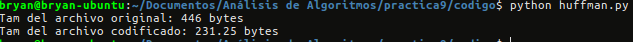
\includegraphics[width=10cm,height=1.5cm]{imagenes/5.png}
	\centering
	\caption{Tamaño de la compresión.}
	\centering
\end{figure}

 \newpage
	Pseudocódigo del algoritmo de decodificación:
	\lstset{language=python, breaklines=true, basicstyle=\footnotesize}
	\lstset{numbers=left, numberstyle=\tiny, stepnumber=1, numbersep=10pt}
	\begin{lstlisting}
def decode(encode,i):
  word=""
  txt=""
  for line in i:
    for char in line:
      word+=char
      k=findEncode(encode,word)
      if k!=-1:
        node=encode[k]
        txt+=node[0]
        word=""

  return txt
	\end{lstlisting}
	  
La función \textbf{decode}, decodifica el archivo original comparando cada cadena de bits, con la codificación cargada a partir del archivo \textbf{codificacion.txt}. El algoritmo va formando cadenas de bits hasta que alguna coincidencia sea encontrada en la tabla de codificación, de ser así, coloca el símbolo correspondiente en la cadena de retorno, la cual al final de la ejecución del algoritmo, contendrá el contenido del texto original.

\textbf{Input.}\\
Archivo \textbf{archivo\_codificado.txt} y archivo \textbf{codificacion.txt}.\\

\textbf{Output.}\\
La figura 6, muestra el contenido del archivo \textbf{archivi\_decodificado.txt}.\\
\begin{figure}[H]
	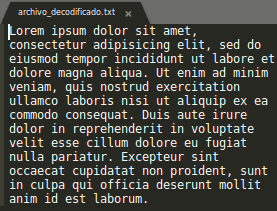
\includegraphics[width=10cm,height=5.5cm]{imagenes/6.png}
	\centering
	\caption{archivo\_decodificado.txt.}
	\centering
\end{figure}
	  
\newpage		
\section{Conclusiones}
Esta práctica se me hizo muy interesante, sobretodo, porque la implementación del algoritmo de Huffman no es nada sencilla. Las estructuras de datos implementadas son un tanto complejas y el procedimiento del algoritmo tiene cierto grado de complejidad. Tuve problemas al momento de realizar la función del algoritmo de Huffman, pero lo pude solucionar implementado el módulo de python llamado \textit{heapq}, el cual por medio de una cola de prioridad, me permitió emular los árboles binarios que se requieren para el algoritmo.\\
Desde mi punto de vista, la parte más sencilla de la práctica fue decodificar el archivo, ya que la codificación hecha previamente no permite la ambigüedad en la compresión.\\
Sin duda los algoritmo Greedy son una gran herramienta para poder alcanzar la solución óptima de un problema, sin embargo, no siempre se pueden aplicar, ya que hay problemas en los que es necesario buscar un enfoque dinámico para poder dar con la solución óptima.

\newpage

\section{Bibliografía}

[1] https://es.wikipedia.org/wiki/Algoritmo\_voraz\\

[2] https://es.wikipedia.org/wiki/Codificación\_Huffman\\
	
\end{document}